\documentclass[flenqn, 14pt]{extarticle}

\usepackage[14pt]{extsizes}
\usepackage{amssymb}
\usepackage{amsmath}
%%\setlength{\mathindent}{0pt}
\usepackage{stmaryrd}

\usepackage{graphicx}
\usepackage{epstopdf}

\usepackage{mathtext} % Русские буквы в формулах
\usepackage{array}

\usepackage{longtable}
\usepackage[left=2cm,right=2cm,
    top=2cm,bottom=2cm,bindingoffset=0cm]{geometry}
    
\usepackage{latexsym} %Включает latex пакеты
\usepackage[T2A]{fontenc} %Подключает поддержку кодировок, отличных от латиницы.
\usepackage[utf8]{inputenc} %Указывает, что текст будет вводится в utf8 кодировке.
\usepackage[russian]{babel} %Подключает интернациональный паке babel.
\usepackage{setspace}
\pagestyle{plain} \onehalfspacing

\usepackage{ccaption}
\captiondelim{. }

\begin{document}
\begin{center}
\section*{Измененный и переоцененный Reduceron (Редуцерон)}
\end{center}
\begin{center}
Мэтью Нейлор (Mettew Naylor) и Колин Рансиман (Colin Runciman) \\
Департамент информатики, Йоркский университет, Йорк, Северный Йоркшир, Великобритания \\
(e-mail: \{mfn,colin\}@cs.york.ac.uk)
\end{center}

\section*{Реферат}
Представлена новая версия специалированного процессора для исполнения ленивых функциональных программ. Этот процессор - Редуцерон - использует параллельную память и динамический анализ для увеличения скорости исполнения и реализован, используя перенастраиваемое аппаратное обеспечение. По сравнению с более традиционными реализациями функционального языка, нацеленные на стандартный RISC процессор, работающий на том же перенастраиваемом аппаратном обеспечении, Редуцерон предлагает существенное улучшение производительности во время выполнения.

\section{Введение}
Эффективное выполнение высокоуровневых функциональных программ на традиционных компьютерах - большой вызов. Необходимы сложные техники для использования архитектурных возможностей, разработанных для низкоуровневой императивной модели исполнения. Более того, традиционные компьютеры имеют ограничения при исполнении функциональных программ. Для примера, ширина канала памяти ограничена последовательным обменом маленькими частями информации. Исполняющие устройства, основанные на редукции графов, производят интенсивные операции по созданию и уничтожению выражений в памяти. Каждая такая операция требует последовательного исполнения множества машинных инструкций, не из-за наличия врожденных зависимостей в данных, а из-за архитектурных решений в традиционных компьютерах.

Все это стимулирует идею компьютеров, специально спроектированных для соответствия нуждам высокоуровневым функциональных языков - примерно как графические ускорители (GPU) созданы для соответствия задачам компьютерной графики. С помощью обеспечения минимального набора возможностей, специально заточенных для исполнения функциональных программ, такой \textit{специализированный компьютер} может быть не только быстрым, но и простым с достоинствами, такими как: более полная верификация и более низкое потребление энергии. Это не новая идея. В 1980х и 1990х проводилась 15-ти летняя серия конференций ACM (\textbf{Association of Computing Machinery} - Ассоциация Вычислительной Техники) - \textit{Функциональные Языки программирования и Компьютерная Архитектура}. Исходя из раздельных инициатив, существовал целый симпозиум занятый только графо-редукционными машинами (Фазель (Fasel) \& Келлер (Keller) 1987), и крупный производитель компьютеров изготовил прототип графо-редукционной машины (Чивел (Scheevel) 1986). Но процесс прозводства нового экзотического аппаратного обеспечения был медленный и неопределенным. Из-за крупных продвижений в компиляции для еще более больших, быстрых и дешевых массовых машин, идея специализированного аппаратного обеспечения для функциональных языков вышла из моды.

\textbf{Реконфигуриемое аппаратное обеспечение.} В наши дни ситуация немного другая. \textit{Программируемая пользователем вентильная матрица} (ППВМ или FPGA) сильно уменьшило усилия и необходимость в экспертизе в разработке специализированного аппаратного обеспечения. FPGA содержит тысячи параллельных логических блоков, которые могут быть настроены по желанию разработчика с помощью программных инструментов. Они широко распространены и представляют из себя развитую технологию сами по себе. 

Недостатоком применения FPGA является то, что они обычно имеют гораздо более низкие максимальные рабочие частоты, чем соответствующие специально разработанные кристаллы - это цена, которую мы платим за перенастраиваемость. Следовательно, для достижения хорошей производительности, используя FPGA, необходимо значительно использовать параллелизм. 

\textbf{Редуцерон.} В данной статье мы представляем специализированную машины для последовательной редукции графа - the Reduceron  (Редуцерон) - реализованный на FPGA. Мы основываемся на нашей предыдущей работе по этой же теме (Нейлор (Naylor) \& Рансиман (Runciman) , 2008) и представляем новый дизайн, который показывает пятикратное улучшение производительности.

Примечательная особенность нашего нового дизайна является то, что каждое из его шести семантических правил редукции производится за один такт. Все необходимые транзакции памяти, необходимые для выполнения редукции, производятся параллельно. Редуцерон производит в среднем 0.55 ручных редукций (hand-reductions) на каждый такт. Ручная редукция - это редукция, которую программист бы производил при \textit{ручном} выполнении трека программы; она включает в себя применения функций и анализ частности (case analysis), но не включает редукции машинного уровня такие как обновление и размотка (unwinding). 

Другая важная разработка в нашем новом дизайне - это использование динамического анализа, позволяющего выполнять \textit{избегание обновления} (update avoidance) и \textit{предсказательное вычисление примитивных выражений} (speculative evaluation of primitive redexes), каждая из которых приводит к значительному улучшению производительности. На традиционных компьютерах накладные расходы во время исполнения такого динамического анализа будут непомерно высокими, но на FPGA он дешевый и простой в реализации.

\textbf{Вклад.} В целом, было сделано следующее: \\
\textbf{Глава 2.} Точное описание компилятора Редуцерона, включая уточнения для кодирования конструкторов по Скотту (Scott encoding of constructors), используемое для компилирования частных выражений (case expressions) и связанное с различными проблемами эффектиности.

\textbf{Глава 3.} Рабочая семантика машины конкретизации шаблонов, лежащая в основе реализации Редуцирона.

\textbf{Глава 4.} Подробное описание как каждое семантическое правило редукции реализовано в один такт, используя FPGA.

\textbf{Глава 5.} Расширения в семантику для поддержки (1) динамического анализа разделяемости, используемого для избегания нежелательных обновлений кучи, и (2) динамическое определение примитивных выражений, позволяющее произвести предсказательную редукцию таких выражений во время конкретизации тела функции. 

\textbf{Глава 6.} Сравнительная оценка реализации Редуцерона с другими реализациями функционального языка.

\textbf{Расширения.} Это статья является расширенной версией статьи для конференции (Нейлор (Naylor) \& Рансимэн (Ranciman), 2010). Главные новые дополнения следующие:
\begin{itemize}
\item Рисунок 2 добавлен для формализации схемы компиляции Редуцерона.
\item Глава 4.3 расширена новыми деталями агоритма разделения шаблонов.
\item Глава 6.1 расширена сравнением Редуцерона с традиционным компилируемой реализации функционального языка, нацеленной на \textit{Компьютер с Сокращенным Набором Комманд} (RISC), работающим на той же FPGA. (Это наиболее значительное новое добавление, отраженное добавление слова "переоцененный" к названию статьи).
\item Глава 6.9 расширена большим количеством деталей начальных экспериментов со статическими предположениями о примитивных выражениях (static primitive-redex speculation (PRS)).
\item Главы 6.10, 6.12, 6.13 и 6.14 добавлены для расширенного обсуждения связанных работ.
\end{itemize}

\begin{figure}[t]
\centering
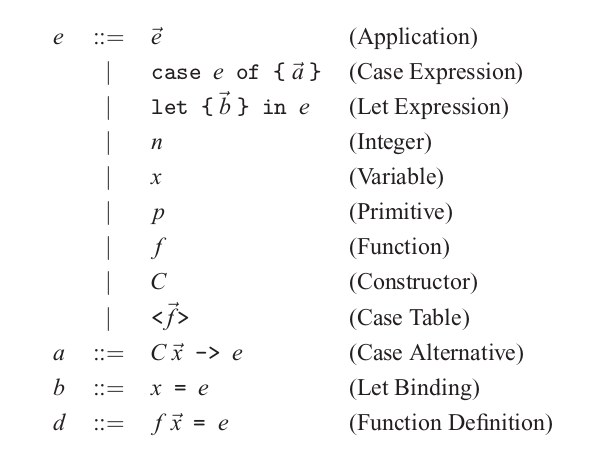
\includegraphics[scale=0.4]{core_syntax}
\label{fig:core_syntax}
\caption{Синтаксис ядра языка F-lite.}
\end{figure}

\section{Компиляция}
Эта секция определяет набор уточнений, которые приводят программу, написанну на ленивом языке программирования F-lite, к форме, известной как \textit{шаблонный код} (template code), которую Редуцерон может исполнять.

\subsection{Исходный язык}
F-lite является ядровым ленивым функциональным языком, близкий к подмножествам как Haskell так и Clean. Синтаксис F-lite представлен на рис.~\ref{fig:core_syntax}.

\textbf{Частные выражения (case expressions).} Частные выражения представлены в упрощенной форме, которая может быть получена с помощью компилятора шаблонного поиска (pattern match compiler), такого как тот, который определен в Peyton Jones (1987). Шаблоны в частных выражениях являются конструкторами, примененными к нулю или более переменным. Каждое частное выражение содержит альтернативу для каждого конструктора расматриваемого в выражении типа.

\textbf{Примитивы.} Мета-переменная \textit{p} обозначает символ примитивной функции. Все применения примитивных функций полностью насыщены (т.е. они не могут частично применяться, можно подать только столько переменных, сколько арность примитивной функции). Редуцерон реализует только малый набор примитивных операций, не полный набор традиционного процессора, например, отсутствуют операции с числами с плавающей запятой. В примитивы, используемые в данной статье, включаются (+), (-) и (<=).

\textbf{Main.} Каждая программа содержит определение главной функции \textit{main = e}, где e является выражением, которое вычисляется в целочисленное n; результат выполнения программы - значение n.

\textbf{Таблицы частных случаев (Case tables).} Отметим необычную конструкцию для таблиц частных случаев $<\overrightarrow{f}>$. Таблицы частных случаев не пишутся в исходных программах, а появляются во время компиляции - смотри Главу 2.4.

\textbf{Примеры.} Ниже представлены два примера для определения функции. Первая соединяет два списка и вторая высчитывает треугольные числа.

\begin{verbatim}
append xs ys = case xs of
  { Nil -> ys ; Cons x xs -> Cons x (append xs ys) }
  
tri n = case (<=) n 1 of
  { False -> (+) (tri ((-) n 1)) n ; True -> 1 }
\end{verbatim}

\subsection{Терминология}
\textbf{Длина применения (Application length).} \textit{Длина} применения $e_1 \ldots e_n$ есть $n$. Для примера, длина применения \textit{append xs ys} - 3.

\textbf{Смешанные выражения (Compound expression) и атомарные выражения (atomic expressions).} Применения, частные выражения и выражения объявления (let expressions) являются смешанными. Все другие выражения являются атомарными.

\textbf{Плоские выражния (Flat expression).} Плоское выражение - это атомарное выражение или применение $e_1 \ldots e_n$, в котором каждое $e_i$ для $i \in [1 \ldots n]$ является атомарным выражением. Для примера, \textit{append xs ys} является плоским выражением, но \textit{tri ((-) n 1)} не является.

\textbf{Граф выражения (Expression graph).} Выражение объявления:
$$
let \; \{ x_1 = e_1 ; \ldots ; x_n = e_n \} \; in \; e
$$
является графом выражения тогда и только тогда, когда $e$ является плоским выражением и каждое $e_i$ для $i \in [1 \ldots n]$ также является плоским выражением. Графы выражений являются ограниченными А-нормальными формами (Flanagan et al., 1993). 

\textbf{Индекс конструктора и арность.} Каждый конструктор $C$ типа данных с $m$ конструкторами связан с уникальным индексом в диапазоне $1 \ldots m$. Точнее, индекс конструктора является его позицией в отсортированном в алфавитном порядке списке всех конструкторов данного типа. Например, стандартный тип данных для списка имеет два конструктора: \textit{Cons} имеет индекс 1 и \textit{Nil} имеет индекс 2. Конструктор с индексом $i$ обозначается как $C_i$, и арность конструктора $C$ обозначается как $\#C$.

\subsection{Примитивные применения}
В ленивом языке применение примитивной функции, такой как (+), (-) или (<=) требует специальной обработки: целочисленные аргументы должны быть полностью вычислены перед тем как применение будет редуцировано. Одним из простых подходов является трансформация бинарного примитивного применения с помощью правила:
\begin{equation} \label{eq:rule_primitive_applications}
p \; e_0 \; e_1 \rightarrow e_1 \; (e_0 \; p)
\end{equation}

вместе с правилом редукции во время исполнения:
\begin{equation} \label{eq:reduce_primitive_applications}
n \; e \rightarrow e \; n
\end{equation}

для полностью вычисленного целочисленного литерала $n$. Для иллюстрации данного подхода, рассмотрим выражение \textit{(+) (tri 1) (tri 2)}. Благодаря применению правила (\ref{eq:rule_primitive_applications}) во время компиляции, выражение трансформируется в \textit{tri 2 ((tri 1) (+))}. Во время исполнения, редукция проводится следующим образом:

\begin{align*}
& tri \; 2 \; ((tri \; 1) \; (+)) & \{ tri \; 2 \; \text{вычисляется в} \; 3 \} & \\
& = 3 \; ((tri \; 1) \; (+)) & \{ \text{Правило (2)} \} & \\
& = (tri \; 1) \; (+) \; 3 &  \{ tri \; 1 \; \text{вычисляется в} \; 1 \} & \\
& = 1 \; (+) \; 3 & \{ \text{Правило (2)} \} & \\
& = (+) \; 1 \; 3
\end{align*}

После трансформации с помощью правила (\ref{eq:rule_primitive_applications}), \textit{tri} выглядит как:
\begin{verbatim}
tri n = case 1 (n (<=)) of
  { False -> n (tri (1 (n (-))) (+)) ; True -> 1 }
\end{verbatim}

В Главе 5 мы представляем более эффективные техники для работы с примитивными применениями.

\subsection{Частные применения (Case expressions)}
Эта глава описывает как компилируются частные выражения. Сперва расмотрим кодирование по Скотту (Scott, 1968) недавно переоткрытое Jansen et al (2007). После этого дадим несколько уточнений для данного кодирования.

\textbf{Кодирование по Скотту/Янсену.} Первый шаг кодирования - генерация для каждого конструктора $C_i$ типа данных с $m$ конструкторами определения функции:
\begin{equation} \label{eq:scott_encoding_1}
C_i \; x_i \ldots x_{\#C_i} \; k_1 \ldots k_m = k_i \; x_1 \ldots x_{\#C_i}
\end{equation}

Идея в том, что каждый конструктор данных $C_i$ закодирован как функция, которая берет $\#C_i$ аргументов конструктора и $m$ продолжений (continuations). Функция, кодирующая конструктор $C_i$, передает аргументы конструктора i-тому продолжению Для примера, конструкторы списка трансформируются в следующие функции:

\begin{verbatim}
Cons x xs c n = c x xs
Nil       c n = n
\end{verbatim}

Теперь частное выражение следующей формы:
\begin{equation} \label{eq:scott_encoding_2}
case \; e \; of \; \{ \; C_1 \; \vec{x}_1 \; \rightarrow e_i ; \ldots ; \; C_m \; \vec{x}_m \rightarrow e_m \; \}
\end{equation}

трансформируется в:
$$
e \; (alt_1 \;  \vec{v}_1 \; \vec{x}_1 ) \ldots (alt_m \;  \vec{v}_m \; \vec{x}_m )
$$
, где $\vec{v}_i$ - свободные переменные, появляющиеся в i-той частной альтернативе и каждый $alt_i$ для $i \in [1 \ldots m]$ имеет определение:

$$
	alt_i \; \vec{v}_i \; \vec{x}_i = e_i
$$

Для примера, функция \textit{append} трансформируется в:
\begin{verbatim}
append xs ys = xs (consCase ys) (nilCase ys)
consCase ys x xs = Cons x (append xs ys)
nilCase  ys      = ys
\end{verbatim}

Заметьте, что применение \textit{nilCase} можно редуцировать во время компиляции. Это следствии того, что конструктор \textit{Nil} имеет арность 0.

\textbf{Другой пример.} Теперь посмотрим на пример крупнее - вычисление базовых арифметических выражения.
\begin{verbatim}
eval x y e = case e of {
  Add n m -> (+) (eval x y n) (eval x y m);
  Neg n   -> (-) 0 (eval x y n);
  Sub n m -> (-) (eval x y n) (eval x y m);
  X       -> x;
  Y       -> Y;
}
\end{verbatim}

После преобразования и подстановки (in-lining) нулевых случаев, мы имеем:
\begin{verbatim}
eval x y e = e (add x y) (neg x y) (sub x y) x y
add  x y n m = (+) (eval x y n) (eval x y m)
neg  x y n   = (-) 0 (eval x y n)
sub  x y n m = (-) (eval x y n) (eval x y m)
\end{verbatim}

Посмотрите на объемное тело \textit{eval}: оно содержит три вложенных применений функций и несколько повторяющихся ссылок на $x$ и $y$. В типичной реализации функционального языка программирования большие тела функций более дороги для создания, чем маленькие.

\subsection*{Улучшение 1} 
Вместо того, чтобы частично применять каждую альтернативную функцию в частном выражении к свободным переменным, которые относятся к данной функции, мы можем определить каждую такую функцию так, чтобы она брала \textit{все} свободные переменные, появляющиеся в \textit{любой} альтернативе. Альтернатива в частном выражении может просто игнорировать переменные, которые ей не нужны. Так что вместо этого трансформируем частное выражение в:
$$
e \; alt_1 \ldots alt_m \; \vec{v}
$$ 
, где $\overrightarrow{v}$ - объединение свободных переменных в каждой альтернативы частного выражения, и каждая $alt_i$ для $i \in [1\ldots m]$ имеет определение:
$$
alt_i \; \vec{x}_i \; \vec{v} = e_i
$$
Каждая функция-альтернатива в частном выражении теперь сначала берет аргументы конструктора, потом свободные переменные, а не наоборот. Для иллюстрации, \textit{append} теперь выглядит как:
\begin{verbatim}
append xs ys = xs consCase nilCase ys
consCase x xs ys = Cons x (append xs ys)
nilCase       ys = ys
\end{verbatim}

И \textit{eval} преобразуется в:
\begin{verbatim}
eval x y e = e add neg sub xCase yCase x y
add   n m x y = (+) (eval x y n) (eval x y m)
neg   n   x y = (-) 0 (eval x y n)
sub   n m x y = (-) (eval x y n) (eval x y m)
xCase     x y = x
yCase     x y = y
\end{verbatim}

Новые тела \textit{append} и \textit{eval} \textit{не содержат} вложенных применений функций и повторяющихся ссылок. Очевидным недостатком является то, что мы должны предоставить функции для 0-арных альтернатив конструкторов \textit{nilCase}, \textit{xCase} и \textit{yCase}. Но наше следующее улучшение подготавливает способ для нивелирования цены такого применения этих функций.

\subsection*{Улучшение 2}
Теперь у нас есть длинный ряд прилегающих констант в теле \textit{eval}. Для того, чтобы представить эти коснтанты эффективным образом (смотри Главу 2.7), мы помещаем их в \textit{таблицу частных случаев} (case table). Частные выражения трансформируются в:
$$
e \; <alt_1, \ldots, alt_m> \; \vec{v}
$$
и каждый конструктор $C_i$ кодируется как:
$$
C_i \; x_1 \ldots x_{\#C_i} \; t = (t \; ! \; i) \; x_1 \ldots x_{\#C_i}
$$
, где $t \; ! \; i$ возвращает i-ый элемент таблицы частных случаев $t$.

\subsection*{Улучшение 3}
Вычислитель может обрабатывать конструкторы эффективнее, чем обобщенные определения функций. Мы можем предоставить следующее правило редукции для конструкторов:
$$
C_i \; e_1 \ldots e_{\#C_i} \; t \; \rightarrow \; (t \; ! \; i) \; e_1 \ldots e_{\#C_i}
$$
Данное правило заменяет конструктор функцией-альтернативой в частном выражении с помощью поиска в таблице частных случаев, используя индекс конструктора. Однако, это правило \textit{также} теряет аргумент t. В результате реализация будет вынуждена перемещать аргументы конструктора вниз по стеку. Правило редукции, которое не требует перемещения аргументов:
\begin{equation} \label{eq:reduce_rule_constructors}
C_i \; e_1 \ldots e_{\#C_i} \; t \; \rightarrow \; (t \; ! \; i) \; e_1 \ldots e_{\#C_i} \; t
\end{equation} 

Чтобы принять во внимание факт того, что t не было сброшено, определение функций-альтернатив принимает форму:
$$
alt_i \; \vec{x}_i \; t \; \vec{v} = e_i
$$

Финальная версия \textit{append}:
\begin{verbatim}
append xs ys = xs <consCase, nilCase> ys
consCase x xs t ys = Cons x (append xs ys)
nilCase       t ys = ys
\end{verbatim}

Аргумент t просто игнориуется функциями-альтернативами. Финальная версяи \textit{tri}:
\begin{verbatim}
tri n = 1 (n (<=)) <falseCase, trueCase> n
falseCase t n = n (tri (1 (n (-))) (+))
trueCase  t n = 1
\end{verbatim}

В главах 3.3 и 4.7 мы увидим как эти улучшения позволяют принимать эффективные решения на уровне реализации.

\subsection{Подстановка}
Определение \textit{append} больше не является явно рекурсивным. Это последствие разделения альтернатив частного выражения на определения новых функций. Однако, прямая рекусрия легко восстановима: просто подставить (in-line) определение \textit{append} в теле \textit{consCase}.
\begin{verbatim}
consCase x xs t ys =
  Cons x (xs <consCase, nilCase> ys)
\end{verbatim}

Эта трансформация демонстрирует следующее общее правило подстановки: \textit{подставлять насыщенные приложения функций с плоскими телами}. Подстановка плоского выражения \textit{e} часто является большим выигрышем, так как она устраняет редукцию, и \textit{e} часто не больше чем, применение, которое оно заменяет.

\subsection{Графы выражений}
В целях реализации обычно удобно делать структурный граф тел функций явным с помощью преобразования их к графам выражений (Глава 2.2). Это достигается с помощью трех правил преобразования.
\begin{enumerate}
\item Поднятие вложенных применений в привязки объявлений (let bindigns):
$$
e_1 \ldots (e_i) \ldots e_n \rightarrow let \; \{ \; x = e_i \; \} in e_1 \ldots x \ldots e_n
$$
, где $e_i$ является применением или выражением объявления, и $x$ - новая переменная.
\item Поднятие выражений объявлений из тел выражений объявления:
$$
let \; \{ \; \vec{b}_0 \; \} \; in \; (let \; \{ \vec{b}_1 \} \; in \; e) \rightarrow let \; \{ \; \vec{b}_0 ; \vec{b}_1 \; \} \; in \; e
$$
\item Поднятие выражений объявления из привязок объявлений:
$$
let \{ \ldots ; x = let \; \{ \vec{b} \} \; in \; e_0 ; \ldots \} \; in \; e_1 \rightarrow \\
	let \; \{ \ldots; \vec{b} ; x = e_0 ; \ldots \} \; in \; e_1
$$
\end{enumerate}

Данные правила принимают на себя переименование переменных, чтобы удостовериться в отсуствии затенения переменных (variable shadowing). Для иллюстрации последнего, определение \textit{falseCase} становится:
\begin{verbatim}
falseCase t n =
  let {x0 = tri x1 (+); x1 = 1 x2; x2 = n (-)} in n x0
\end{verbatim}

Легко увидеть число и длину применений в графе выражений. Например, \textit{falseCase} содержит четыре применения и ее самое длинное применение, \textit{tri x1 (+)}, имеет длину три.

\subsection{Шаблонный код}
Каждое определение функции теперь имеет форму:
$$
f \; x_0 \ldots x_n = let \; \{ \; v_0 = e_0; \ldots ; v_m = e_m \} \; in \; e
$$
, где каждое выражение плоское (и список привязок объявлений может быть пустым). Это представление очень близко к \textit{шаблонному коду}, который фактически может быть непосредственно выполнен на Редуцероне. Мы определим шаблонный код как тип данных Haskell, прокладывая путь к семантике исполнения, которая определена в Главе 3. Для того, чтобы выдвинуть это определение семантики на первый план и провести различия между ней и кодом F-lite, мы предваряем данные определения символом '>'.

В шаблонном коде программа определна как список шаблонов.
\begin{verbatim}
> type Prog = [Template]
\end{verbatim}

Шаблон представляет определение функции. Оно содержит \textit{арность}, \textit{хребтовое применение (spine application)} и список \textit{вложенных применений (nested applications)}.
\begin{verbatim}
> type Template = (Arity, App, [App])
> type Arity = Int
\end{verbatim}

Хребтовое определение содержит тело выражения объявления, относящиеся к определению графа выражения, и вложенные определения содержат привязки выражения объявления. Применения плоские и представлены как списки атомов. 
\begin{verbatim}
> type App = [Atom]
\end{verbatim}

Атом - это маленький помеченный кусок нерекурсивных данных.
\begin{verbatim}
> data Atom =
>    FUN Arity Int -- Функция с арностью и адресом
>  | ARG Int       -- Ссылка на аргумент функции
>  | PTR Int       -- Указатель на применение
>  | CON Arity Int -- Конструктор с арностью и индексом
>  | INT Int       -- Целочисленная константа
>  | PRI String    -- Имя примитивной функции
>  | TAB Int       -- Таблица частных случаев
\end{verbatim}

После применения преобразований, описанных в Главах от 2.3 до 2.6, F-lite программы могут быть компилированы в шаблонный код Редуцерона с помощью схемы компилирования, описанной на рисунке \ref{fig:compilation_sheme}. Следующие параграфы описывают, менее формально, как таки программы компилируются в шаблонный код.

\begin{figure}[t]
\begin{align*}
D \llbracket f_i \; x_0 \ldots x_n = let \left\lbrace v_0 = e_0; \ldots; v_m = e_m \right\rbrace in \; e \; \rrbracket &= \left( n+1, A_\sigma \llbracket e \rrbracket, \left[ A_\sigma \llbracket e_0 \rrbracket, \ldots, A_\sigma \llbracket e_m \rrbracket \right] \right) \\
\textbf{where} \; & & \\
\sigma &= [x_0 \mapsto \textit{ARG} \; 0, \ldots, x_n \mapsto \textit{ARG} \; n, \\
       &\;\;\;\;\;\;  v_0 \mapsto \textit{PTR} \; 0, \ldots, v_m \mapsto \textit{PTR} \; m] \\
\\
A_\sigma \llbracket e_0 \ldots e_n \rrbracket &= [E_\sigma \llbracket e_0 \rrbracket, \ldots, E_\sigma \llbracket e_n \rrbracket ] \\
\\
E_\sigma \llbracket n \rrbracket &= \textit{INT} \; n \\
E_\sigma \llbracket p \rrbracket &= \textit{PRI} \; p \\
E_\sigma \llbracket v \rrbracket &= \sigma \; v \\
E_\sigma \llbracket C_i \rrbracket &= \textit{CON} \; \#C_i \; i \\
E_\sigma \llbracket f_i \rrbracket &= \textit{FUN} \; \#f_i \; i \\
E_\sigma \llbracket \langle f_i, f_{i+1}, \ldots, f_j \rangle \rrbracket &= \textit{TAB} \; i
\end{align*} 
\label{fig:compilation_sheme}
\caption{Схема компиляции из трансформированных F-lite программ в шаблонный код Редуцерона. Схема D применяется к определениям функций; схема A применяется к применениям; схема E применяется к атомарным выражениям; и $\sigma$ определяет соответсвие из переменных в атомы.}
\end{figure}

\textbf{Функции.} Дан список определений функции:
$$
f_0 \; \vec{x}_0 = e_0, \ldots, f_n \; \vec{x}_n = e_n
$$
Каждый идентификатор фукнции $f_i$, появляющийся в $e_0 \ldots e_n$, транслируется в атом \textit{FUN \#f i}, где \textit{\#f} - арность функции $f$.

\textbf{Аргументы.} В каждом определении $f \; x_0 \ldots x_n = e$ каждая переменная $x_i$, появляющаяся в $e$, транслируется в атом \textit{ARG i}.

\textbf{Переменные в привязках выражения объявления.} В каждом графе выражений:
$$
let \; \{ \; x_0 = e_0 ; \ldots ; x_n = e_n \} \; in \; e
$$
Каждый $x_i$, появляющаяся в $e$, $e_0\ldots e_n$ транслируется в атом \textit{PTR i}.

\textbf{Целочисленные, примитивы и конструкторы.} Целочисленная константа $n$, примитив $p$ и конструктор $C_i$ транслируются в атомы \textit{INT n}, \textit{PRI p} и \textit{CON \#$C_i$ i} соответственно.

\textbf{Таблицы частных случаев.} Дан лист определений функции:
$$
f_0 \; \vec{x}_0 = e_0, \ldots, f_n \; \vec{x}_n = e_n
$$

Каждая таблица частных случаев $\langle f_i, \ldots, f_j \rangle$, появляющаяся в $e_0 \ldots e_n$, транслируется в атом \textit{TAB i}. Договоримся, что функции в каждой таблице частных случаев определены по соседству в шаблонном коде.

\textbf{Пример.} Рассмотрим следующую программу, включающую функцию \textit{tri}:
\begin{verbatim}
main          = let { } in tri 5
tri       n   = let { x = n (<=) } in 1 x <falseCase, trueCase> n
falseCase t n = let { x0 = tri x1 (+); x1 = 1 x2; x2 = n (-) } in n x0
trueCase  t n = let { } in 1
\end{verbatim}

Шаблонный код для данной программы представлен ниже:
\begin{verbatim}
> tri5 :: Prog
> tri5 = [ (0, [FUN 1 1, INT 5], [])
>        , (1, [INT 1, PTR 0, TAB 2, ARG 0],
>              [[ARG 0, PRI "(<=)"]])
>        , (2, [ARG 1, PTR 0],
>              [[FUN 1 1, PTR 1, PRI "(+)"],
>               [INT 1, PTR 2],
>               [ARG 1, PRI "(-)"]])
>        , (2, [INT 1], []) ]
\end{verbatim}

Заметим, что каждое определение функции соответствует шаблонну, представленный как кортеж длины три. Первая компонента каждого шаблона - арность функции. Вторая и третья компоненты представляют тело выражения объявления у функции и привязки выражения объявления соответственно. Функции без привязок отображаются в шаблоны с пустой третьей компонентой. Функции, применения и аргументы обознаются по позиции. Например, атом \textit{FUN 1 1} в первом шаблоне представляет вызов функции арности 1, которая находится по индексу 1 в списке шаблонов (в данном случае, вызов функции \textit{tri}). И атом \textit{PTR 2} в третьем шаблоне является указателем на применение по индексу 2 в списке применений, соответствующему привязкам выражения объявления (в данном случае, применение называется \textit{x2}).

\section{Рабочая семантика}
Данная глава определяет \textit{рабочую семантику малых шагов (small-step operational semantics} для Редуцерона. Существует две главных причины привести семантику:
\begin{itemize}
\item Точно определить как работает Редуцерон;
\item Подчеркнуть низкоуровневый параллелизм, присуствующий в редукции графа, испольуземой в Редуцероне.
\end{itemize}
Мы нашли очень удобной прямую запись в Haskell данной семантики: перед тем, как приступать к низкоуровневой реализации, можно проанализировать сложность и производительность различных дизайнерских решений и оптимизаций.

Сердцем определения семантики является функция перехода состояния:
\begin{verbatim}
> step :: State -> State
\end{verbatim}

, где состоянием является четверка, содержащая программу, кучу, редукционный стек и стек обновлений.
\begin{verbatim}
> type State = (Prog, Heap, Stack, UStack)
\end{verbatim}

Куча моделируется как список приложений и может быть проиндексирована с помощью адреса кучи:
\begin{verbatim}
> type Heap = [App]
> type HeapAddr = Int
\end{verbatim}

Элемент в куче может быть изменен с помощью функции обновления:
\begin{verbatim}
> update :: HeapAddr -> App -> Heap -> Heap
> update i a as = take i as ++ [a] ++ drop (i+1) as
\end{verbatim}

Реудкционный стек также моделирвется как список узлов, для которого верхний элемент стека является первым и нижный элемент является последним.
\begin{verbatim}
> type Stack = [Atom]
> type StackAddr = Int
\end{verbatim}

Также присуствует стек обновлений:
\begin{verbatim}
> type UStack = [Update]
> type Update = (StackAddr, HeapAddr)
\end{verbatim}

Значение программы $p$ определено с помощью \textit{run p}, где:
\begin{verbatim}
> run :: Prog -> Int
> run p = eval initialState
>   where initialState = (p, [], [FUN 0 0], [])

> eval (p, h, [INT i], u) = i
> eval s = eval (step  s)
\end{verbatim}

Начальное состояние вычислителя содержит программу, пустую кучу, стек с одним элементом - вызовом \textit{main} и пустой стек обновлений. Главный шаблон имеет арность 0 и мы считаем, что этот шаблон находится по адресу 0. Для демонстрации этого, \textit{run tri5} выводит 15. В следующих подглавах определена центральная функция \textit{step}.

\subsection{Редукция примитивов}

\end{document}